\documentclass{article}
\usepackage[utf8]{inputenc}

\title{Wireless}
\author{ngrmarco }
\date{February 2020}

\usepackage{natbib}
\usepackage{graphicx}

\begin{document}

\maketitle

\section{Introduction}

This paper will cover the protocols used in Mobile Ad-hoc NETworks (MANETs) to deliver packets over a distributed and unreliable topology.
These protocols have been divided in two groups: proactive and reactive, depending on the amount of overhead messages sent and the data cached.
But a bigger difference lays between link-state and distance vector routing strategies.

Babel (RFC6126) offers a good theoretical approach to define a MANET.
Babel is a proactive, distance vector based protocol and uses sequence numbers to update the routes.
It will be compared with other protocols, like DSDV and AODV,  from which Babel learns.

\section{sigle!}

MANET
DSDV
AODV

\section{Mobile Ad-hoc NETworks}

Mobile Ad-hoc NETworks, from now on MANETs, are networks made by mobile nodes that communicates with each other over wireless links.
Being mobile means that there is no predefined topology on which nodes can rely.


Being wireless links between nodes must be seen as unreliable, and ever changing.
Distributed algorithms for routing packets already exists in the today internet network, but instead of faulty link they face the problem of routing packets over the whole internet (the Border Gateway Protocol is the protocol used in the communication between and inside Autonomous Systems, that we see as Internet Service Providers).

Some protocols born from completely wireless environment, others from hybrid ones. This brings little differences in the challenge that are posed to the developers.

A stronger characterization comes from the battery supply nature of wireless mobile nodes, we can see protocols especially made for very constrained devices (bluetooth, zigbee). These often rely on different kind of nodes, defining coordinator, routers and leaf.

I find way more interesting protocols that works in a more p2p manner.

\section{The Protocols}


We can see a MANET as a graph, as shown in figure \ref{fig:graph}.


Delivering a packet means finding a path between sender and receiver wherever, assuming that it exists.

There are two big distinction that we can make to categorize the existing algorithms:

\begin{itemize}
    \item Proactive or Reactive
    \item Distance vector or Link State
\end{itemize}{}

\subsection{Proactive or Reactive}

A node can have a view of the network from the messages it receives. Whenever a message is to be sent the path might be ready or require recalculation.
If no messages have recently came from a node it might either be silent or unreachable.

The trade-off is between:
\begin{itemize}
    \item overhead on the channel
    \item readiness to deliver messages
\end{itemize}{}

Proactive protocols are meant to be always ready to send a messages, and periodically send broadcast messages to keep an updated view of the network.
Reactive protocols compute 

\subsubsection{Proactive}
Proactive protocols are characterized by a periodic broadcast HELLO messages.

May be sent with a limited Time To Live (TTL), like in BATMAN:
messages with TTL of 1 are broadcasted every half second,
messages with TTL of 2 or 3 are broadcasted every 2 or 4 second
messages with TTL of 255 (infinity) are broadcasted every 11 second, and that is the worst case time to recover 

This have the effect of giving nearer nodes a better knowledge of the network. 

Being broadcast messages they are not rebroadcasted twice, hence nodes must keep track of the recent broadcasts done. 
In this category we can find protocols like OLSR BABEL DSDV BATMAN



\subsubsection{Reactive}
Reactive protocols generates no overhead if there isn't any message to send.

Information required to the message delivery may be requested just before sending the message.

I have found few information on reactive protocols, because the most popular protocols today are proactive.
The reasons behind a reactive protocol may be, in my humble opinion, that network doesn't change that often or that it changes so often that it is not worth to keep track of its changes if not necessary.
In the former case, with a quite stable network, one can use protocols like OSPF.
And I suppose that these protocols have smaller success because the latter case, is not so common.


In this section we can find AODV and DSR


\subsection{Distance vector or Link State}
These two categories can be found with different names:
Link State aka source routing, it means that every node knows the whole topology of the network, and in the message is contained the path it must follow, the routing is made by the sender.

Distance Vector aka Table Routing aka next-hop, it means that every node has a table that describes the best next hop towards any other node in the network

be careful when reading anything, this terms are used interchangeably, and often I have found it confused with the difference between proactive and reactive.


space\\

In practical terms the difference between the two is where the path planning happens:
in Link State it happens on the sender side. it has knowledge of the whole state of the network, and can plan 
When a intermediary node receives a message to forward, it can look in the header to find the next hop.
BATMAN project noted that this has a high computational cost, since whenever a node move EVERY node have to recalculate every best path to every other node.
Then, it noted also that since the planner of the routing is often far from the destination, and may suffer from obsolete information. it causes to increase the HELLO messages and routing loops are frequent.

Distance vector makes use of a algorithm known as Distributed Bellman Ford.
Each node has a table with 3 columns: destination, next hop, metric.


The classical theoretic algorithm is made to calculate best path, but do not takes in consideration that it can change over time.

Route change is the main cause for routing loops. (using metric and bellman ford statically applied assures to have a direct acyclic graph)

To avoid loops generation, ... TODO

DSDV (RFC....) first introduced sequence numbers.

DSDV may go into starvation, and made the seqnum periodically increasing, Babel gives the starved node the option to use loop-risky connection to broadcast a request for new seqnum



Bellman ford works minimizing the cost of the path, having weighted arcs between nodes

\subsection{Metrics}
How much does a link cost?
a lot of metrics have been proposed, like number of hops or link quality or quantity.

number of hops: AODV, or GPS aided routing. Since minor number of hops SEEMS to mean better performance, hence we give every link a fixed weight of 1.


But this is not realistic model. links do not have the same characteristic.
Batman 3 (or 1?) introduce a way to evaluate link quality. it was 2006, wireless link were more unrelaiable than today. we can call this "link quality"
2012 came, and Batman reached version 5, where another metric came out: bandwith, that we can see as "link quantity".

Now, what properties do a metric needs to have?
This is structured by Babel:
-it must be strictly increasing or decreasing


Links are unstable, ok, but how nodes have to measure link quality.
link quality measurmaent alla fine e' la cosa che fa la differenza tra un protocollo efficace e uno no.



BATMAN evolved through different versions, using different metrics.

\begin{frame}{Link evaluation}
Links are unstable, ok, but how nodes have to measure link quality.

OSLR weight all links one, hence it minimize the hops between source. but it happens that direct link may be bad ones.



BATMAN evolved through different versions, using different metrics.

Batman III counts the OMG received to determine 



To ensure that the detected connections allow communication in both directions each B.A.T.M.A.N. node awaits rebroadcasts of its own OGMs from his neighbors within a certain timeframe (bidirectional link check). If the OGMs are not successfully retransmitted the connection is considered too asymetric (unusable) and therefore ignored.

The B.A.T.M.A.N. III algorithm has serious problems when it comes to asymetric links. The bidirectional link check tries to limit its impact but the result is far from being perfect. The timeframe in which B.A.T.M.A.N. accepts his own OGMs being rebroadcasted by its neighbor allows to tweak the behaviour. If this timeframe is rather short B.A.T.M.A.N. is very strict on choosing links. This may lead to many ignored links which might be usable in one direction. \textbf{Only symetric connections will be considered}. If the timeframe value is less strict B.A.T.M.A.N. will accept more links but \textbf{tends to route in the wrong direction}.


 B.A.T.M.A.N. IV has been enhanced with the Transmit Quality (TQ) algorithm. 

B.A.T.M.A.N. IV divides a given link quality into 2 distinct parts: receiving link quality and transmit link quality. The receiving link quality expresses the probability of a successful packet transmission towards the node.
%https://www.open-mesh.org/projects/batman-adv/wiki/BATMAN_IV

The local link quality needs to be propagated throughout the network to inform other nodes about the transmit quality. Therefore B.A.TM.A.N. IV introduces a new field called "TQ" which is 1 byte long.

The receiving neighbor will calculate their own local link quality into the received TQ value and rebroadcast the packet. Hence, every node receiving a packet knows about the transmit quality towards the originator node.

 
Although the transmit link quality is most important decision factor B.A.T.M.A.N. IV also keeps track of the receiving link quality. On the WiFi layer every unicast packet has to be acknowledged by the neighbor node to approve the transmission. If this neighbor is not able to sucessfully send his ACKs the WiFi layer considers this transmission to be failed and tries to retransmit until it gives up.



Since a packet loss based metric as used by B.A.T.M.A.N. IV isn't adequate to handle the increasing number devices and link types with little to no packet loss but very different throughput capabilities B.A.T.M.A.N. V uses packet throughput as mesh-wide metric.

Depending on the link type batman-adv is able to determine the throughput automatically:

    wireless: Modern WiFi drivers export the estimated throughput per WiFi neighbor. This value is retrieved on a periodic basis and averaged before propagated in the mesh.
    wired: Most Ethernet capable devices export their theoretical throughput and duplex capabilities via the ethtool API.
    unknown/override: B.A.T.M.A.N. V allows to specify a throughput value per interface via generic netlink. Consequently. B.A.T.M.A.N. V will assume the specified throughput for any neighbor discovered over that interface.
    throughput meter (upcoming): If the throughput can not be queried via some API and is not manually configured, B.A.T.M.A.N. V will run a periodic throughput test with its built-in throughput test protocol.


\end{frame}

Source Routing requires every node to recalculate every path towards every other node every time a link changes.


\subsection{routing loops, black holes}
avoid generating useless messages!



\section{further expansion}
This presentation is over but there are still lot iof things to say!:
Sequence numbers, which are used in babel, aodv, DSDV. to determine if a path needs to be recalculated.
In babed to avoid starvation.

Hierachical networks
Zigbee and bluetooth have an uneven resource distribution, and there are nodes more important than others.
OLSR calculates Multi-relay-Point, even if nodes can have similar resources.

Babel and Batman are flat, and there is no backbone constructed.
At least, until you start talking about gateways to the Internet.
The 

I have talked very little about loop avoidance.
Babel make of this a fundamental argument, while batman in his documentation refers to loop avoidance only in LAN backbones.

every route has a number used to indicate if a route is old



\section{Introduction}

Wireless mesh networks are supposed to route packets in a very harsh environment:

\begin{itemize}
    \item Dynamic topology
    \item No centralized or planned infrastructure
    \item Faulty wireless connections
    \item Asymmetrical link 
\end{itemize}
%Optimal path between nodes must be recalculated often, and must be stored distributedly.

A mesh protocol must:
\begin{itemize}
    \item Maintain path
    \item Route packets
\end{itemize}



\section{Packet routing}


Packet routing can be done in one of this two methodologies :
\\\textbf{Source routing} or \textbf{Table routing}

%\begin{itemize}
%    \item Source routing
%    \item Table routing
%\end{itemize}



Let's take a imaginary world with symmetrical and weighted links
\begin{figure}
  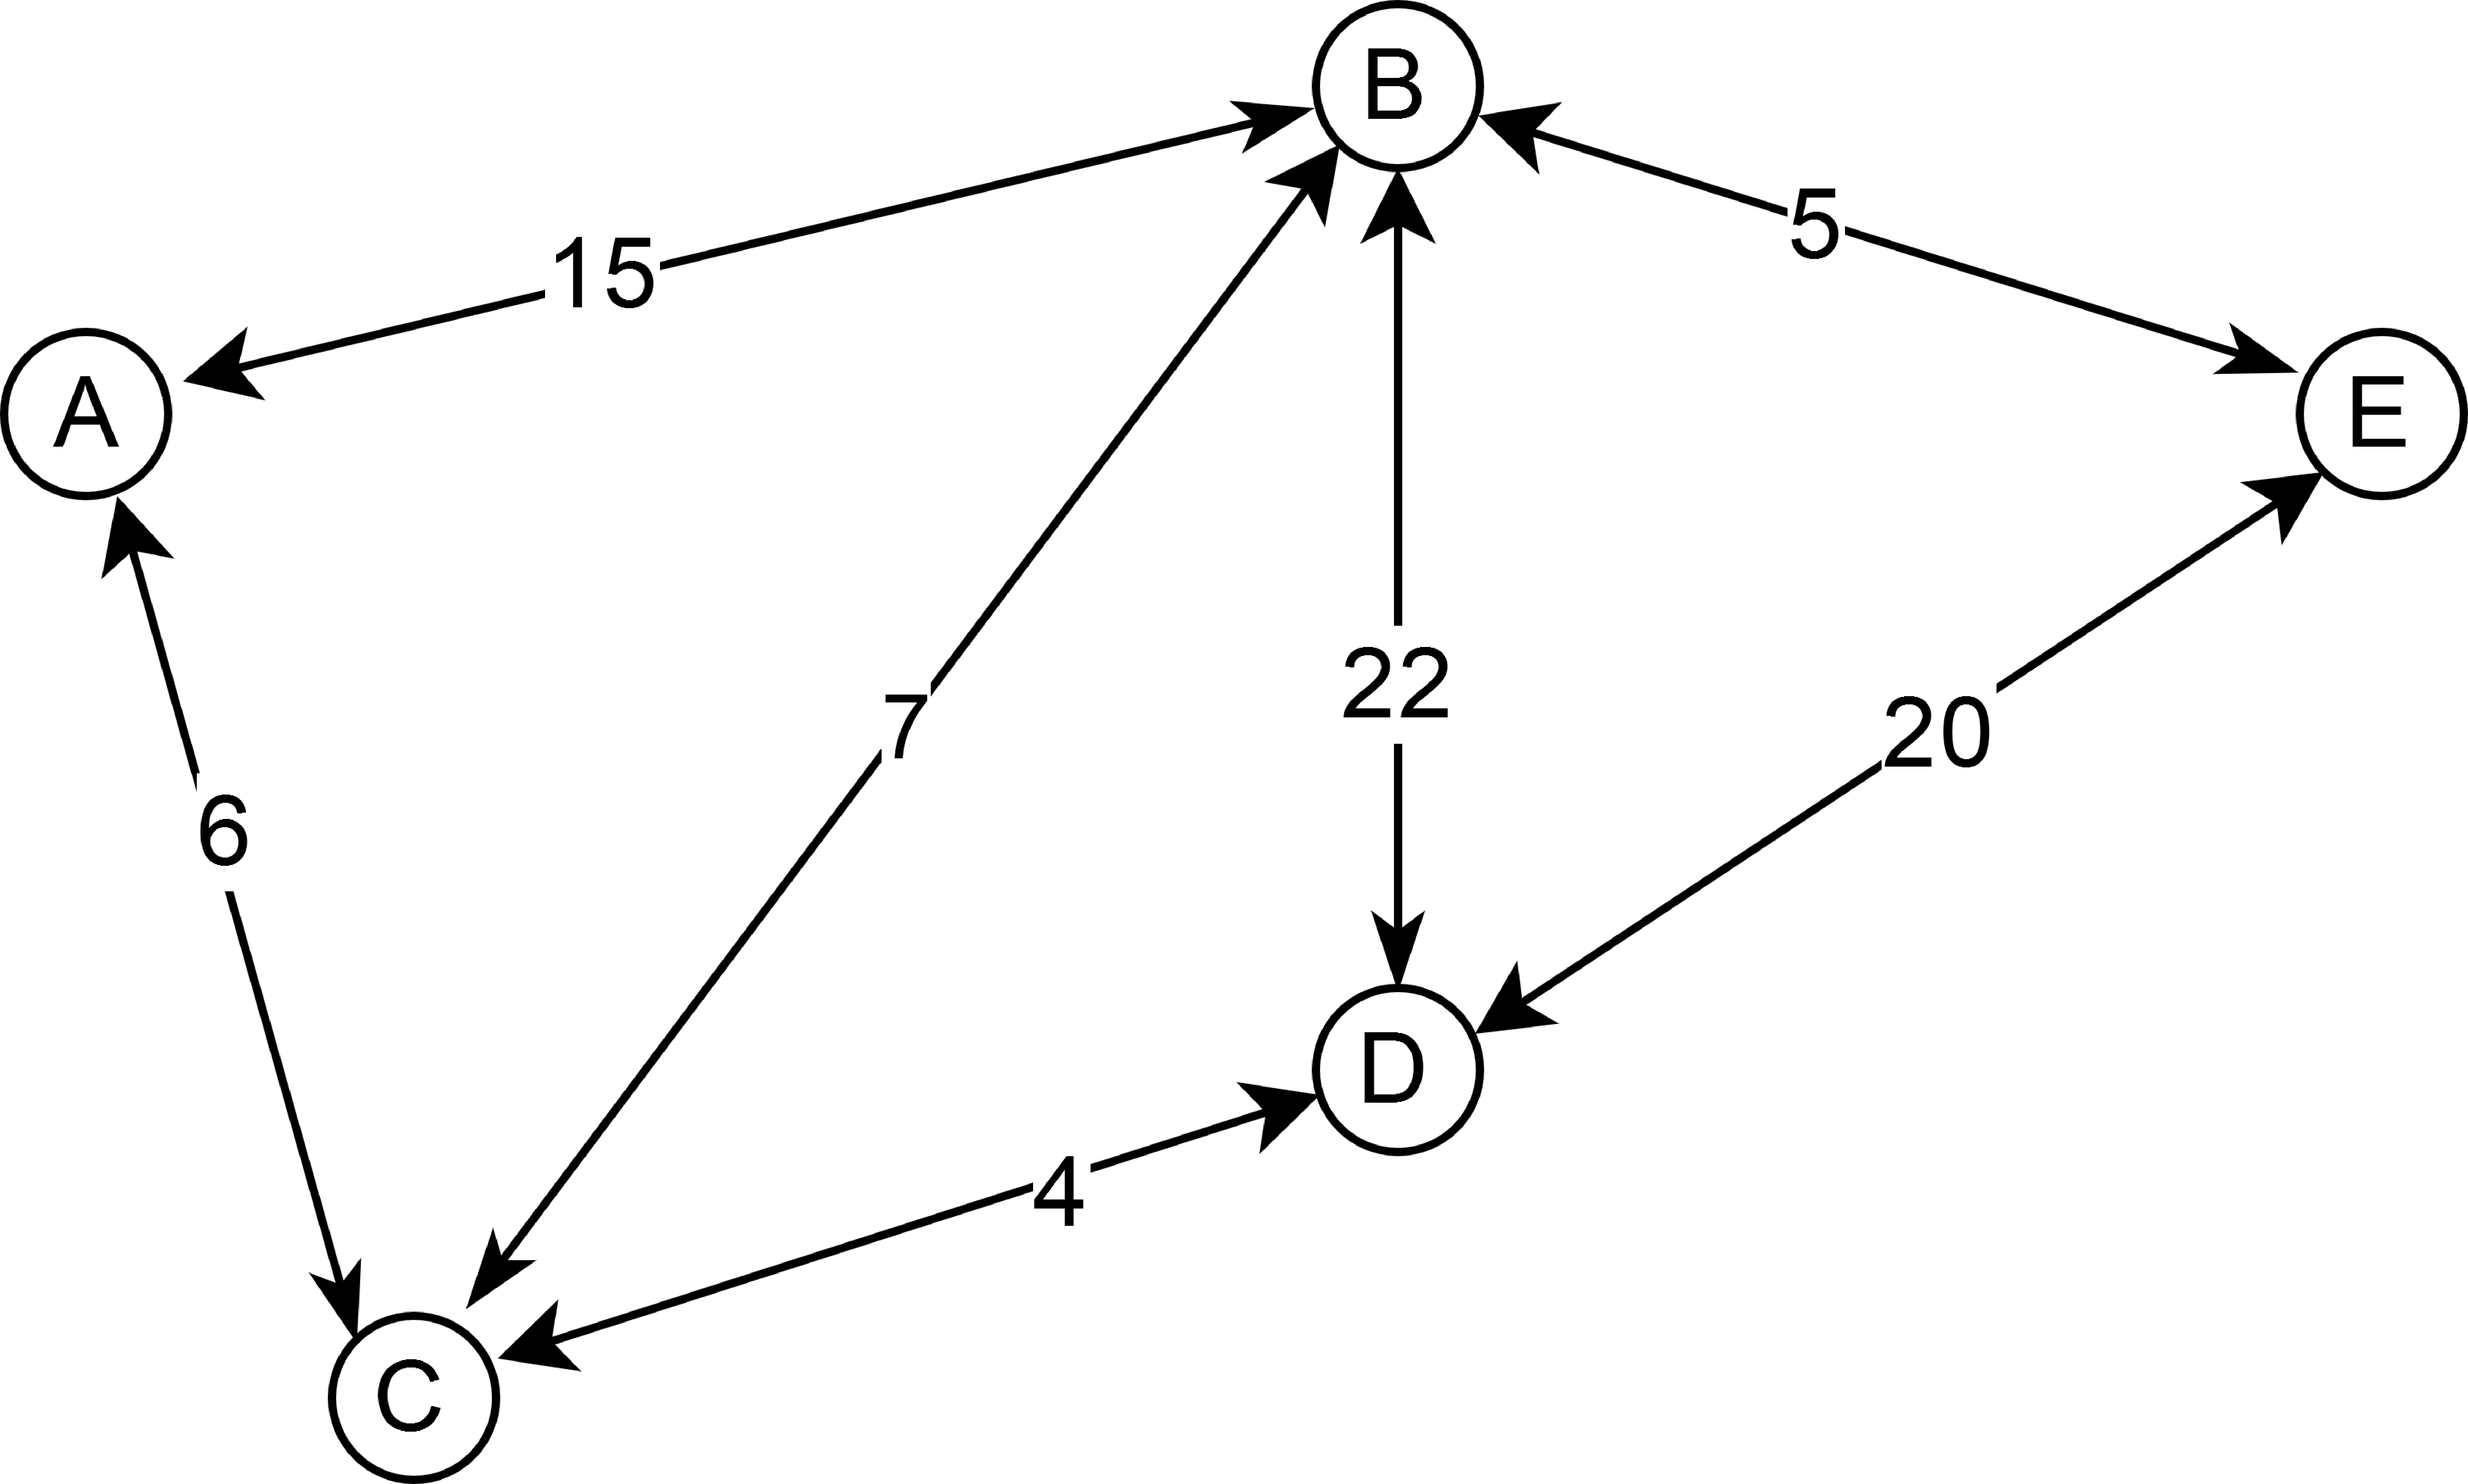
\includegraphics[width=250pt]{img/distributed_graph.pdf}
  %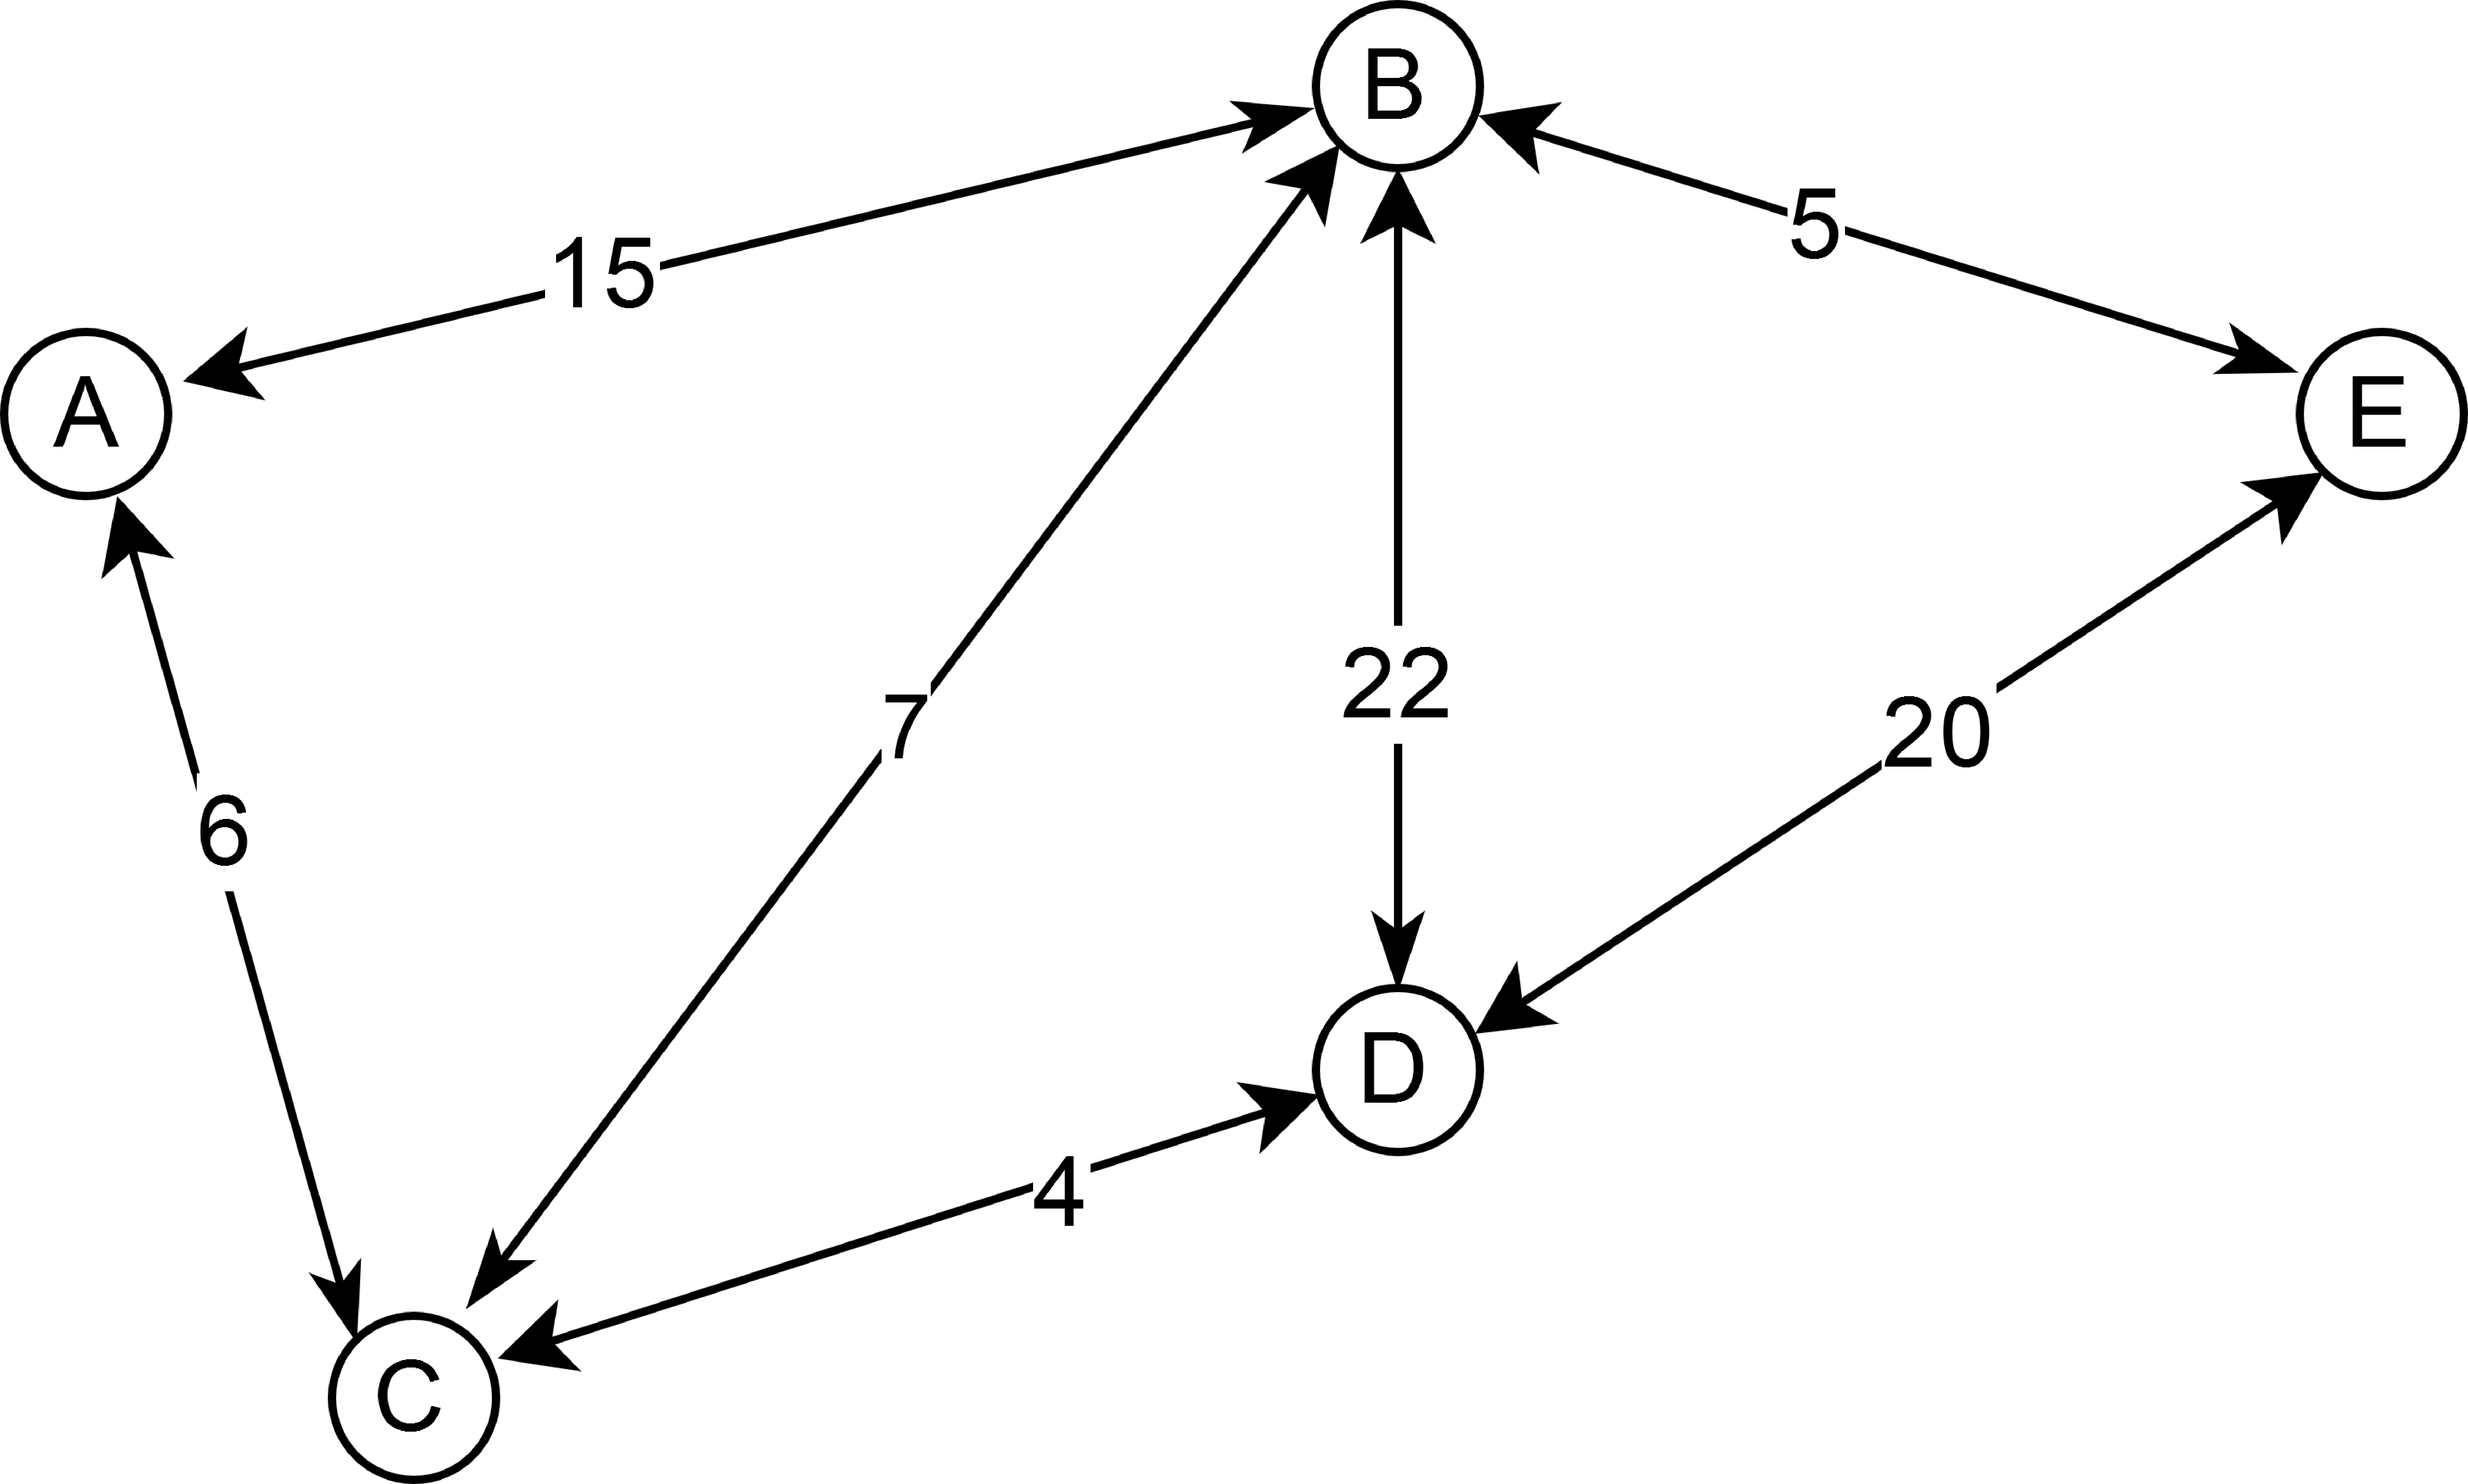
\includegraphics[width=250pt]{img/distributed_graph.pdf}
  \caption{Distributed network}
  \label{fig:dg}
\end{figure}

\begin{figure}
  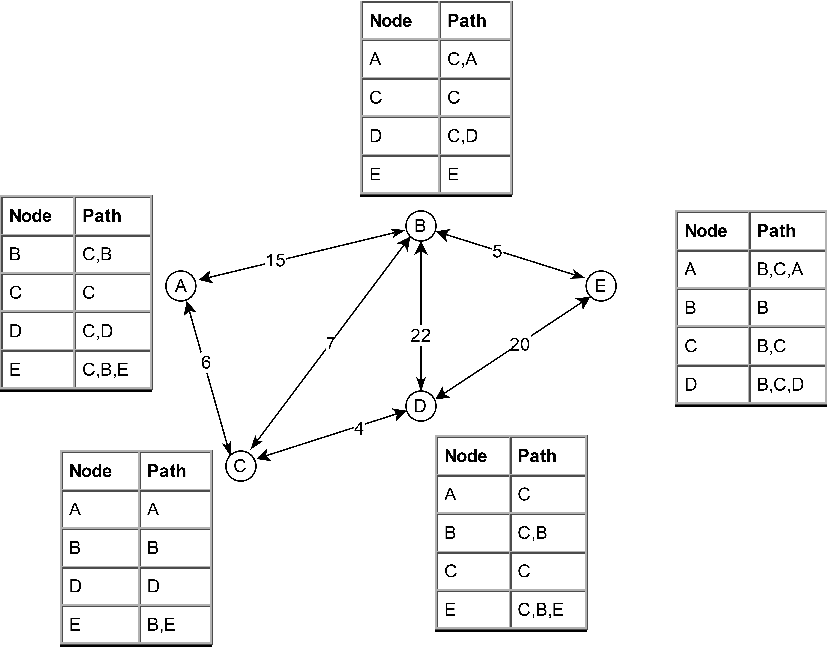
\includegraphics[width=250pt]{img/LS_routing.pdf}
  %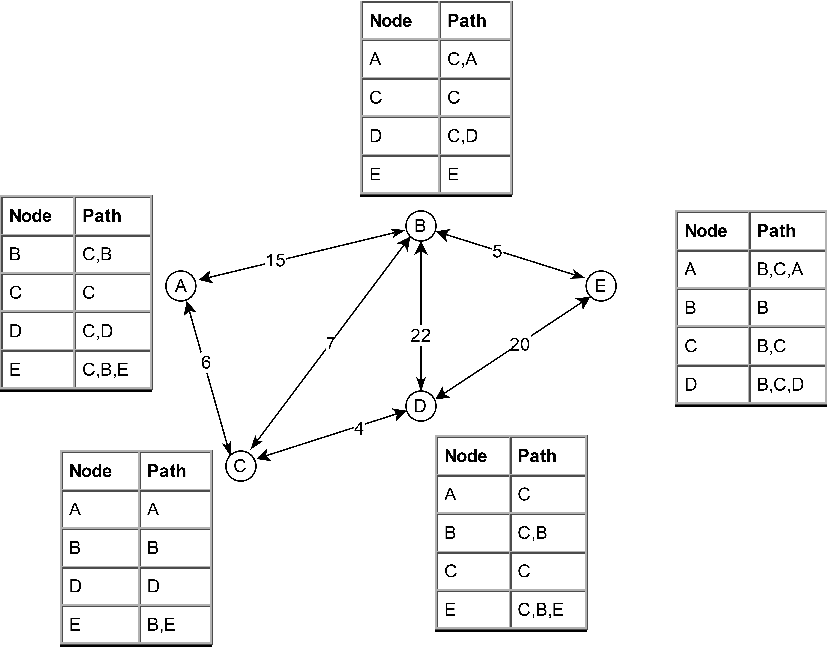
\includegraphics[width=250pt]{img/LS_routing.pdf}
  \caption{Source Routing}
  \label{fig:LS}
\end{figure}

\begin{figure}
  \includegraphics[width=250pt]{img/LS_routing_msg1.pdf}
  \caption{Source Routing}
  \label{fig:LSmsg_1}
\end{figure}

\begin{figure}
  \includegraphics[width=250pt]{img/LS_routing_msg2.pdf}
  \caption{Source Routing}
  \label{fig:LSmsg_2}
\end{figure}

\begin{figure}
  \includegraphics[width=250pt]{img/LS_routing_msg3.pdf}
  \caption{Source Routing}
  \label{fig:LSmsg_3}
\end{figure}

\begin{figure}
  \includegraphics[width=250pt]{img/DV_routing.pdf}
  \caption{Table Routing}
  \label{fig:DV}
\end{figure}

\begin{figure}
  \includegraphics[width=250pt]{img/DV_routing_msg1.pdf}
\end{figure}

\begin{figure}
  \includegraphics[width=250pt]{img/DV_routing_msg2.pdf}
\end{figure}

\begin{figure}
  \includegraphics[width=250pt]{img/DV_routing_msg3.pdf}
\end{figure}

How path is stored in the distributed network determine how routing is processed:
\begin{itemize}
    \item \textbf{Source routing} or \textbf{Link state}:  
        Every Node know the \underline{path} towards every other node.
        Every node runs the algorithm  to determine the best routes to every other node.
    \item \textbf{Table Routing} or \textbf{Distance Vector}:
        Every node knows the \underline{next hop} towards every other node.
        The Network runs a distributed algorithm called distributed bellman ford.
\end{itemize}

Path maintenance is the act of \underline{giving a weight} to links.
%Every node is directly connected to a subset of the nodes of the network.
%They must decide which link is best, for a given destination.

This weight of a link may measure:
\begin{itemize}
    \item \textbf{Distance} in number of hops
    \item \textbf{Link quality}, percentual of delivered packets (which is quite of a cross layer problem)
    \item \textbf{Link quantity}, bandwith
    \item \textbf{Geographical position}

\end{itemize}


The network is perceived through \textbf{message flooding}, in the form of \underline{searches for a specific node}, or \underline{self-announcement}.

Link evaluation can be done following tow possible philosophy:
\begin{itemize}
    \item \textbf{Reactive}:  Also known as \textbf{On-Demand}.
        When a node wants to send a packet it floods the network for a route discovery.
    \item \textbf{Proactive}: Periodic messages to keep tracks of changes.
        Every node is always ready to send new messages. 
    \item Anything in the middle is considered a hybrid solution
\end{itemize}

\begin{center}
\begin{tabular}{ c | c |  c }
 . & Proactive & Reactive \\ 
 \hline
 Table Routing & BATMAN, BABEL, DSDV & AODV \\  
  \hline
 Source Routing & OLSR & DSR \\
\end{tabular}
\end{center}


BATMAN is a mesh protocol

it had a lot of versions

it is Proactive and table driven
Every node periodically self-announce itself with so-called Originator Messages (OGM)
OGM are rebroadcasted by neighbours.
OGM have a Time To Live, a limit to the maximum number of hops that it can travel. 



\begin{figure}
    \centering
        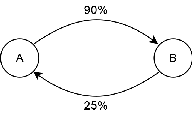
\includegraphics[width=5cm]{img/Asymetric.pdf}
    \qquad
        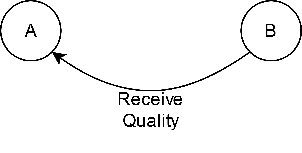
\includegraphics[width=5cm]{img/ReceiveQuality.pdf} 
    \label{fig:example1}
%\end{figure}
%\begin{figure}
    \centering
        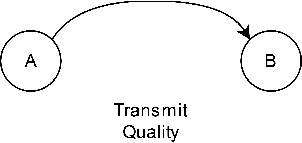
\includegraphics[width=5cm]{img/TransmitQuality.pdf} 
    \qquad
        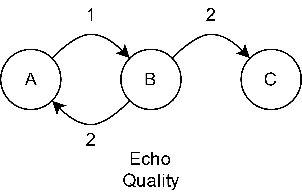
\includegraphics[width=5cm]{img/EchoQuality.pdf} 
    \label{fig:example}
    \caption{referred to A}
    
\end{figure}

\begin{figure}
  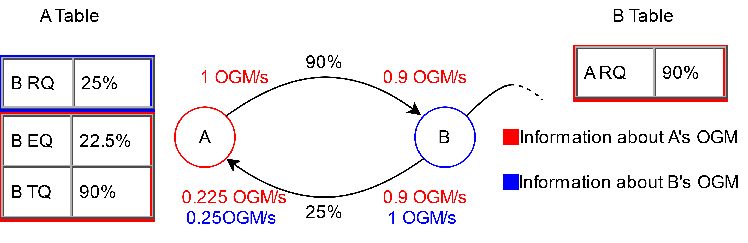
\includegraphics[width=300pt]{img/A-OGM.pdf}
  \caption{Data calculated on the A's OGM received from B, and B's rebroadcasts heard by A}
  \label{fig:calc}
\end{figure}

TQ = EQ / RQ

This represent BATMAN 4, the fifth version is based on bandwidth (quantity) to manage mixed networks too.


\begin{figure}
  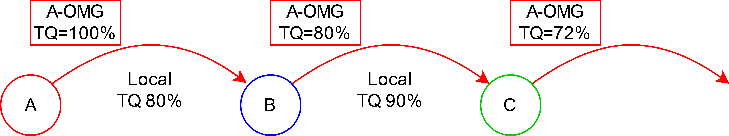
\includegraphics[width=250pt]{img/A-OGM-multi.pdf}
  \caption{Transmit Quality Propagation.}
  \label{fig:DVdsaf}
\end{figure}


Possible arguments as expansion:
\begin{itemize}
    \item Hierachical networks
    \item loop avoidance
    \item sequence numbers
\end{itemize}



%https://www.open-mesh.org/projects/open-mesh/wiki/The-olsr-story












%\bibliographystyle{plain}
%\bibliography{references}
\end{document}
